% Copyright 2007 by Till Tantau
%
% This file may be distributed and/or modified
%
% 1. under the LaTeX Project Public License and/or
% 2. under the GNU Public License.
%
% See the file doc/licenses/LICENSE for more details.


\lecture[review]{Sum-up and review}{lecture-body}

\date{29 April 2015}


\begin{document}

\begin{frame}
  \maketitle
\end{frame}


\begin{frame}\frametitle<presentation>{Outline}
  \tableofcontents
\end{frame}

\section{General principles}

%%%%%%
\begin{frame}{General Principles}

  \begin{itemize}
    \item Always look at, and think about, the data.
    \item Correlation is not causation (consider confounding factors).
    \item Sample size is like a magnifying glass, it lets you see smaller effect sizes,
    \item  ... but statistical significance does not imply real-world importance
    \item Nonindependent observations can drastically mislead you.
    \item If the sampling distribution is not close to Normal, use a distribution-free test.
  \end{itemize}

\end{frame}

\begin{frame}{Descriptive statistics}
    Simple \alert{summaries} of the data:
    \begin{itemize}
        \item \structure{location:} mean, median
        \item \structure{spread:} SD, IQR
        \item proportion of variance explained by group
        \item correlation coefficient ($r$)
        \item \ldots etcetera.
    \end{itemize}

    \vspace{2em}

    Often, we think of these as \structure{estimates} of some unobserved \structure{parameter}.
\end{frame}


\begin{frame}{Parameters, and their estimates}
    There are two basic ways to think about the ``parameters'' we estimate:
    \begin{description}
        \item[real:] properties of some large population we are sampling from.
            \pause
        \item[imaginary:] properties of a statistical model we are using to describe the data.
    \end{description}
    \vspace{2em}
    \pause

    \begin{quote}
            All models are wrong but some are useful.\\
            \hfill \textit{--George Box}
    \end{quote}
    \pause


    \begin{quote}
        \small
               \ldots it does not seem helpful just to say that all models are wrong. 
               The very word \emph{model} implies simplification and idealization. 
               The idea that complex physical, biological or sociological systems 
               can be exactly described by a few formulae is patently absurd. 
               The construction of idealized representations that capture important stable aspects of such systems is, 
               however, a vital part of general scientific analysis and statistical models, 
               especially substantive ones, do not seem essentially different from other kinds of model. 
               \\
               \hfill \textit{--David Cox}
    \end{quote}
\end{frame}

\section{Hypothesis testing}

\begin{frame}{Confidence intervals}
    Statistical results should be accompanied by \alert{context}:\\
    What is the margin of error for the parameter estimate?
    \pause

    \vspace{2em}

    A 95\% \alert{confidence interval} is constructed so that \\
    if you do many experiments,\\
    and for each construct a confidence interval,\\
    the true parameter will fall in the confidence interval \\
    95\% of the time.
    \pause

    \vspace{2em}

    In this framework, the true parameter \\
    \alert{either is, or isn't} in the CI -- \\
    we \structure{cannot say} that the probability \\
    the true parameter is in a \alert{given} CI is 95\%.
    \pause

    \vspace{2em}

    \structure{How?} Related to the $\alpha$ of hypothesis testing.
\end{frame}

\begin{frame}{Example:}

    In a random sample of 100 eggs from a chicken farm,
    the average eggshell thickness is $\bar y= 0.35$mm,
    with standard deviation $s=0.03$mm.  
    Find a 95\% CI for the population mean thickness $\mu$.

    \vfill

    In a random sample of 96 eggs from a chicken farm,
    there are $y=8$ brown eggs.
    Find a 95\% CI for the population proportion of brown eggs, $p$.

    \vfill
    
\end{frame}

\begin{frame}{Necessary sample size}
    In a random sample of 100 eggs from a chicken farm,
    the average eggshell thickness is $\bar y= 0.35$mm,
    with standard deviation $s=0.03$mm.  
    About how big a sample would we need
    to estimate the population mean thickness $\mu$
    to within 0.001mm, with 95\% confidence?

    \vfill

    In a random sample of 96 eggs from a chicken farm,
    there are $y=8$ brown eggs.
    About how big a sample would we need
    to estimate the population proportion $p$
    to within 5\%, with 95\% confidence?

    \vfill
    
\end{frame}

\begin{frame}{Hypothesis testing}
    \alert{``How reasonable is it that these results are just due to noise?''}

    \begin{description}
        \item[these results:] A (descriptive) test statistic.  
        \item[due to noise:] A null hypothesis.
        \item[how reasonable:] The distribution of the test statistic if the null hypothesis is true. 
    \end{description}

    \vspace{2em}
    \pause

    The \structure{$P$-value} is the probability \\
    of obtaining a test statistic \\
    at least as extreme as the one that was observed\\
    under the null model.

    \vspace{2em}
    \pause
    (The alternative hypothesis informs the choice of test statistic,\\
    and how we use its distribution to find a $P$-value.)

\end{frame}

\begin{frame}{Practice}

    Explain, concretely, what the $P$-value means for a two-sample $t$ test
    for a difference in means.
    \vfill

    Explain, concretely, what the $P$-value means for a paired-sample sign test.
    \vfill

    Critique this statement: ``The $P$-value is the probability of the data.''
    \vfill
    
\end{frame}
    
\begin{frame}{Conclusion of a hypothesis test:}
    \begin{itemize}
        \item[$H_0$:] There observed result is just due to (this specific model of) random chance.
        \item[$H_A$:] Something else (interesting) must be going on.
    \end{itemize}
    \pause
    \vfill

    Pick a \alert{significance level}, $\alpha$.  If
    \begin{description}
        \item[$P > \alpha$] We do not have good evidence that $H_0$ is not true\\
            (``fail to reject the null'')
        \item[$P \le \alpha$] We have good statistical evidence \\
            that $H_0$ is not true,
            (``reject the null'')\\
            supporting the idea that $H_A$ is true
    \end{description}
    at the $1-\alpha$ significance level.
    \pause
    \vfill

    \structure{Note:} if $P$ is \emph{very} small,
    can modify to, e.g.\\
    ``We have very good statistical evidence that $H_0$ is not true.''\\
    \pause
    ``You'd be crazy to think that $H_0$ is true, based on these data.''

\end{frame}

\begin{frame}{``What do you conclude?''}

    A dialogue:
    \begin{itemize}
        \item[] ``What did you learn from your experiment?''
            \pause
        \item[] ``That our data were unlikely under our null hypothesis.''
            \pause
        \item[] ``What the \@\#\$*\@\# does that mean?''
    \end{itemize}
    \pause
    \vspace{2em}

    To answer \structure{``What do you conclude?''},\\
    \alert{translate} results into the context of the problem,\\
    considering:
    \begin{itemize}
        \item the strengths and limitations of the test
        \item the limitations of the data (confounders, observation/experiment, power)
    \end{itemize}


\end{frame}


\begin{frame}{A common mistake}
    \structure{Rule of thumb:}
    on a statistics test, if you are saying something definitively,
    you're probably wrong.

    \begin{center}
        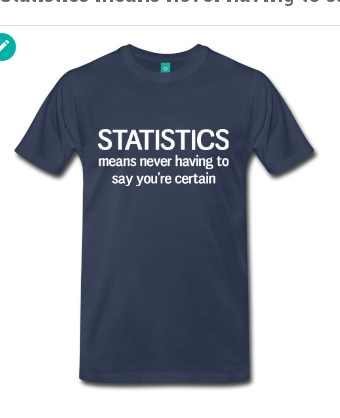
\includegraphics[height=0.7\textwidth]{never-certain}
    \end{center}

    \alert{but} don't go too far the other way \ldots
\end{frame}

\begin{frame}{Practice:}

    \alert{Does infection by malaria increase red blood cell count in western fence lizards?}
    \vfill

    Of \alert{27 field-caught lizards} (15 with malaria, 12 without),
    uninfected lizards had an average count of 130 cells fewer than infected lizards,
    \ldots
    
    \vspace{1em}

    with a standard error of 95 cells ($t_s=1.37$, $\df=24$, \structure{$P>0.1$}).
    \vspace{1em}

    with a standard error of 42 cells ($t_s=3.10$, $\df=24$, \structure{$P<0.01$}).
    \vfill

    Of \alert{27 experimental lizards} (randomly assigned: 15 with malaria, 12 without),
    uninfected lizards had an average count of 130 cells fewer than infected lizards,
    \ldots
    \vspace{1em}

    with a standard error of 95 cells ($t_s=1.37$, $\df=24$, \structure{$P>0.1$}).
    \vspace{1em}

    with a standard error of 42 cells ($t_s=3.10$, $\df=24$, \structure{$P<0.01$}).
    \vfill

\end{frame}

\begin{frame}{Practice:}

    \structure{Does coffee consumption improve mood?}
    \vspace{1em}

    Of one hundred randomly sampled students,
    coffee consumption the previous week
    \ldots
    \vspace{1em}

    showed significant linear correlation 
    with happiness index ($r=0.54$, $P<0.05$).
    \vspace{1em}

    \alert{did not} show significant linear correlation 
    with happiness index ($r=0.14$, $P>0.1$).
    \vfill


    One hundred students were assigned randomly
    to either zero, one, two, or three cups of coffee per day
    for one week;
    coffee consumption 
    \ldots
    \vspace{1em}

    showed significant linear correlation 
    with happiness index ($r=0.54$, $P<0.05$).
    \vspace{1em}

    \alert{did not} show significant linear correlation 
    with happiness index ($r=0.14$, $P>0.1$).
    \vfill

\end{frame}


\section{Tests we have learned}

%%%%%%
\begin{frame}{Tests and CIs}

  \begin{itemize}
    \item two-sample $t$-test
    \item CI for difference in mean
    \item Wilcoxon-Mann-Whitney
    \item paired-sample $t$
    \item paired-sample sign
    \item Wilcoxon signed-rank
    \item CI for estimated proportion
    \item chi-squared for single-sample proportions
    \item two-sample chi-squared
    \item $F$-test for one-way ANOVA
    \item $F$-test for two-way ANOVA
    \item $t$-test for no linear correlation
    \item CI for slope $b_1$
  \end{itemize}

\end{frame}

%%%%%%
\begin{frame}{What you should know for each test}

  \begin{enumerate}
    \item what sort of data the test applies to
    \item what conditions the test needs to be appropriate
    \item how to check the conditions are satisfied
    \item how to formulate the null \& alternative hypotheses
    \item what the test statistic is and how to compute it
    \item what its distribution is under the null hypothesis
    \item how to interpret the result, statistically, and in real-world terms
  \end{enumerate}

\end{frame}

\section{Other notes}

\begin{frame}{A note on randomization}

    Today, you can \structure{almost always} obtain a $P$-value by \alert{simulation}
    \vspace{2em}

    This means: \emph{estimating} the probability rather than looking it up in a table.
    \vspace{2em}
    
    Sometimes, that's the \alert{only way}.

\end{frame}


\begin{frame}{Practice:}
    Given a \alert{fair coin}, a \alert{deck of cards}, a \alert{random number generator}, and a lot of free time, how would you test:
    \vfill

    If fouls in soccer tend to occur closer to the goals (as opposed to uniformly on the field),
    given that the mean distance to the goal for 100 fouls was 15 meters.
    \vfill

    If people with names earlier in the alphabet tend to be taller, given the correlation coefficient between alphabetical position and height for 26 people?
    \vfill

    If right-handers are more common than left-handers, given that 16 out of a sample of 20 are right-handed?
    \vfill

\end{frame}

\begin{frame}{Experimental design}

    An \structure{experiment} differs from an \alert{observational study} \\
    in that the experimenter determines the assignment into groups\\
    (ideally at random).

    \vspace{2em}

    The aim is to remove possible \structure{confounding factors},\\
    which are associated with both $X$ and $Y$, \\
    causing a \structure{spurious association}.

    \vspace{2em}

\end{frame}

\begin{frame}{Practice}

    \structure{Employees who biked to work had significantly lower blood pressure than those who drove.}
    \vfill

    Can we conclude that biking reduces blood pressure?
    \vfill

    How to turn this into an experiment?
    \vfill

\end{frame}

%%%%%%
\begin{frame}{Other concepts}
  
  \begin{itemize}
    \item standard deviation of --
    \item standard error of --
    \item effect size (of difference in means)
    \item back-calculation of necessary sample size to have power to see a certain effect (e.g. for differences in proportion)
    \item the two-way ANOVA model: group means, interaction means, plus noise/variability
    \item correlation: proportion of variance explained
    \item the linear (regression) model: linear conditional mean plus noise/variability
    \item regression: residuals, leverage, influence
  \end{itemize}


\end{frame}

\begin{frame}
    \vfill
    \centering
    {\Large
    Thank you!
    }
    \vfill
\end{frame}

\begin{frame}{Final}
  \begin{center}

      Final: 5/12, 11am-1pm, in this room.

    \vspace{2em}

      Two 8.5"$\times$11" pages, two-sided, of handwritten notes.

    \vspace{2em}

    Bring a calculator (besides your phone).

  \end{center}
\end{frame}

\end{document}


%%%%%%
\begin{frame}{Example}

  Lactate dehydrogenase levels:
  \begin{center}
    \begin{tabular}{crr}
       & Males & Females \\
       \hline
       $n$ & 270 & 264 \\
       $\bar y$ & 60 & 57 \\
       $s$ & 11 & 10
     \end{tabular}

   \vspace{2em}

   \uncover<2->{$t_s=3.3$ and $P=0.001$}
   \end{center}

\end{frame}



%%%%%%
\begin{frame}{Example}

  Body weight:
  \begin{center}
    \begin{tabular}{crr}
       & Males & Females \\
       \hline
       $n$ & 2 & 2 \\
       $\bar y$ & 175 & 143 \\
       $s$ & 35 & 34
     \end{tabular}

   \vspace{2em}

   \uncover<2->{$t_s=0.93$ and $P=0.45$}
   \end{center}

\end{frame}


%%%%%%
\begin{frame}{Example: soil respiration}

  Soil cores from two locations, ``gap'' and ``growth'';
  measured amount of CO${}_2$ released.

  \begin{center}
  \begin{tabular}{l|p{2.5in}}
    growth & 17 \hspace{.25em} 20 \hspace{.25em} 170 \hspace{.25em} 315 \hspace{.25em} 22 \hspace{.25em} 190 \hspace{.25em} 64 \\
    \hline
    gap & 22 \hspace{.25em} 29 \hspace{.25em} 13 \hspace{.25em} 16 \hspace{.25em} 15 \hspace{.25em} 18 \hspace{.25em} 14 \hspace{.25em} 6 \\
  \end{tabular}

    \vspace{2em}

    \structure{Exercise:} help compute the $P$-value.

    \vspace{2em}


    \uncover<2->{
    % wilcox.test( c(17,20,22,64,170,190,315), c(6,13,14,15,16,18,22,29) ) #= 0.015
    $K_1 = 49.5$ and $K_2 = 6.5$ \\
    $0.009 \le P \le 0.014$
    }
  \end{center}

\end{frame}

%%%%%%
\begin{frame}{Example}

    \structure{Example:} hunger rating with and without mCPP.
    \begin{center}
      \begin{tabular}{lrrr}
        \hline
        subject & mCPP & placebo & difference \\ 
        \hline
        1 & 79 & 78 & 1 \\ 
        2 & 48 & 54 & -6 \\ 
        3 & 52 & 142 & -90 \\ 
        4 & 15 & 25 & -10 \\ 
        5 & 61 & 101 & -40 \\ 
        6 & 107 & 99 & 8 \\ 
        7 & 77 & 94 & -17 \\ 
        8 & 54 & 107 & -53 \\ 
        9 & 5 & 64 & -59 \\ 
        \hline
         Mean & 55 & 85 & -30 \\ 
         SD & 32 & 34 & 33 \\ 
         \hline
      \end{tabular}
    \end{center}
\end{frame}

%%%%%%
\begin{frame}{Example}
    Density of nerves at two sites in the intestine in 9 horses:
    \begin{center}
\begin{tabular}{rrrr}
  \hline
 animal & site I & site II & difference \\ 
  \hline
  1 &  50.60 & 38.00 & +12.60 \\ 
  2 &  39.20 & 18.60 & +20.60 \\ 
  3 &  35.20 & 23.20 & +12.00 \\ 
  4 &  17.00 & 19.00 & -2.00 \\ 
  5 &  11.20 & 6.60 & +4.60 \\ 
  6 &  14.20 & 16.40 & -2.20 \\ 
  7 &  24.20 & 14.40 & +9.80 \\ 
  8 &  37.40 & 37.60 & -0.20 \\ 
  9 &  35.20 & 24.40 & +10.80 \\ 
   \hline
\end{tabular}
    \end{center}

\end{frame}


%%%%%%
\begin{frame}{Example}

    Out of 169 women with family histories of breast cancer, 27 had mutations in the BRCA1 gene.

    \pause
    \vspace{2em}

    \alert{Wilson's estimator} gives that around
        \[ \wt p = \frac{27 + 2}{169+4} = .168 \]
    of women with family histories of breast cancer have mutations in BRCA1.

    \vspace{2em}

    The \alert{standard error} of this estimate is
    \[ \SE_{\wt P} = \sqrt{\frac{.168(1-.168)}{169+4}} = .028  \]

    \vspace{2em}

    A \alert{95\% confidence interval} for this proportion is $\wt p \pm 1.96 \times .028$:
    \[ 0.113 < p < 0.223 \]

\end{frame}

%%%%%%
\begin{frame}{Example}

    Colorblindness in females:
    \begin{center}
        \begin{tabular}{r|rrr}
            & observed counts & expected counts & difference\\
            \hline 
            nonmutant & 850 & 840.9 & 9.1 \\ 
            carrier &  146 & 152.2 & -5.8 \\ 
            colorblind & 4 & 6.9 & 2.9  \\
        \end{tabular}
    \end{center}

    \pause
    \vspace{2em}

    \[
        \chi^2_s = \frac{9.1^2}{840.9} + \frac{5.8^2}{152.2} + \frac{2.9^2}{6.9} .
    \]

\end{frame}

%%%%%%
\begin{frame}{Another example}

    By area, 
    40\% is pavement,
    30\% of a Santa Monica parking lot is shiny cars,
    20\% is dull cars,
    and 10\% is other.\\
    \structure{Hypothesis:} birds don't notice what they are pooping on.
    We counted the numbers of bird poops on each in a given day:
    \begin{center}
        \begin{tabular}{rr}
            & observed counts \\
            \hline 
            pavement & 65 \\
            shiny & 77 \\
            dull & 35 \\
            other & 18 \\
            \hline
            total & 195
        \end{tabular}
    \end{center}

\end{frame}


\begin{frame}{Example}


    \begin{center}
        \begin{tabular}{lcc|c}
            & female & male & total \\
            \hline
            HIV test & 9 & 8 & 17 \\
            no HIV test & 52 & 51 & 103 \\
            \hline
            total & 61 & 59 & 120 \\
        \end{tabular}
    \end{center}

    \vspace{1em}

    \structure{Example:}
    \begin{align*}
        \hat \prob\{ \text{HIV test} \} = \frac{17}{120} \\
        \hat \prob\{ \text{HIV test} \vert \text{female} \} = \frac{9}{61} \\
        \hat \prob\{ \text{HIV test} \vert \text{male} \} = \frac{8}{59} \\
    \end{align*}

\end{frame}

%%%%%%
\begin{frame}{The test statistic}

    Observed (expected) counts:
        \begin{center}
            \begin{tabular}{lcc|c}
                & female & male & total \\
                \hline
                HIV test & 9 (8.64) & 8 (8.36) & 17 \\
                no HIV test & 52 (52.36) & 51 (50.64) & 103 \\
                \hline
                total & 61 & 59 & 120 \\
            \end{tabular}
        \end{center}

    \vspace{2em}

    The test statistic is the \alert{same} as $\chi^2_s$:
    \[
        \chi^2_s = \frac{(9 - 8.64)^2}{8.64} + 
            \frac{(8 - 8.36)^2}{8.36} + 
            \frac{(52 - 52.36)^2}{52.36} + 
            \frac{(51 - 50.64)^2}{50.64} = 0.035
    \]
    and there is \alert{one} {degree of freedom}, and $P > 0.2$ \\
    so there is no significant evidence that men and women get tested at different rates.


\end{frame}

%%%%%%
\begin{frame}{Example: Hair and Eye Color}

    In 6,800 German men, hair (columns) and eye (rows) color were:
        \begin{center}
            \begin{tabular}{l|cccc}
                & brown & black & fair & red \\
                \hline
                brown & 438 & 288 & 115 & 16 \\
                grey/green & 1387 & 746 & 946 & 53 \\
                blue & 807 & 189 & 1768 & 47 \\
            \end{tabular}
        \end{center}

\end{frame}

%%%%%%
\begin{frame}{Example I}

\begin{tabular}{ll|rr}
  value & group & $\bar y_i$ & $y_{ij}-\bar y_i$  \\ 
  \hline
3   &  A  &  5.75  &  -2.75      \\
7   &  A  &  5.75  &  1.25       \\
8   &  A  &  5.75  &  2.25       \\
5   &  A  &  5.75  &  -0.75      \\
6   &  B  &  5.00     &  1.00          \\
5   &  B  &  5.00     &  0.00          \\
5   &  B  &  5.00     &  0.00          \\
10  &  B  &  5.00     &  5.00          \\
2   &  B  &  5.00     &  -3.00         \\
3   &  B  &  5.00     &  -2.00         \\
2   &  B  &  5.00     &  -3.00         \\
7   &  B  &  5.00     &  2.00        \\
   \hline
   & SS & 1.5 & 66.75 \\ 
   & df & 1 & 10 \\ 
   & MS & 0.15 & 6.675   \\ 
\end{tabular}

\end{frame}

%%%%%%
\begin{frame}{Summarized, ANOVA-style}

  \begin{center}
    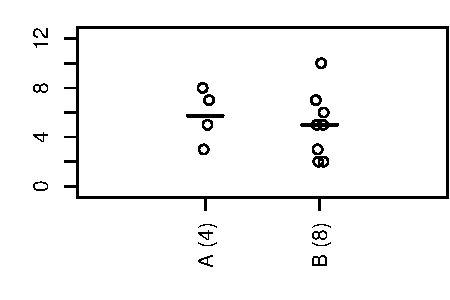
\includegraphics{dots3ex.pdf}

    \vspace{2em}

    \begin{tabular}{lrrr}
      source & df & SS & MS \\
      \hline
      between groups & 1 & 1.5 & 1.5 \\
      within groups & 10 & 66.75 & 6.675 \\
      \hline
      Total & 11 & 68.25 & \\
    \end{tabular}

  \end{center}

\end{frame}

%%%%%%
\begin{frame}{Example of $F$ test}

    Weight gain of lambs on three diets
    \begin{center}
        \begin{tabular}{cccc}
            & diet 1 & diet 2 & diet 3 \\
            \hline
            $n_i$ & 3 & 5 & 4 \\
            $\bar y_i$ & 11 & 15 & 12 \\
            $s_i$ & 4.359 & 4.950 & 4.967 \\
        \end{tabular}
    \end{center}

    \pause

    \begin{center}
        \begin{tabular}{cccc}
            & df & $\SS$ & $\MS$ \\
            between diets & 2 & 36 & 18 \\
            within diets & 9 & 210 & 23.33 \\
            \hline
            total & 11 & 246 & \\
        \end{tabular}
    \end{center}


    \vspace{2em}

    With $df = (2,9)$ and
    \[ F_s = \frac{ 18 }{ 23.33 } = 0.77 , \]
    we find that $P > 0.20$.


    \vspace{2em}

    \pause
    There is not good evidence that diet affects the weight gain of lambs.


\end{frame}

%%%%%%
\begin{frame}{Example: beak size}

    Beak size of finches in different islands:

    { \tiny
\begin{tabular}{c|cccccccccc}
    &   a & a & b & b & c & c & d & d & e & e \\
    &   F & M & F & M & F & M & F & M & F & M \\
    \hline
    & 10.10  &  10.66  & 11.86  &  14.67  &  10.07  & 12.95  &  11.51  &  14.60  &   12.74  & 14.33  \\
    & 9.32   &  13.31  & 14.14  &  14.60  &  10.34  & 11.39  &  13.15  &  13.88  &   13.83  & 16.18  \\
    & 8.42   &  11.88  & 10.72  &  13.97  &  8.42   & 10.86  &  12.93  &  12.48  &   12.91  & 16.42  \\
    & 7.72   &  9.88   & 13.11  &  12.55  &  8.93   & 11.09  &  13.44  &  13.58  &   13.12  & \\
    & 10.04  &  10.85  & 10.14  &  12.60  &  10.20  & 10.95  &  12.91  &  12.76  &          & \\
    & 10.24  &  11.70  & 11.20  &         &   10.93  & 9.39   &  13.08  &  14.51  &          & \\
    & 10.32  &  10.94  & 13.68  &         &   10.29  &        &   12.49  &  14.55  &          & \\
    &        &   9.72   & 12.30  &         &   11.34  &        &   13.19  &  14.81  &          & \\
    &        &   11.03  & 11.12  &         &          &         &   12.54  &  13.20  &          & \\
    &        &   10.87  & 13.24  &         &          &         &   11.29  &  13.83  &          & \\
    &        &   9.55   & 11.99  &         &          &         &   13.45  &  15.05  &          & \\
    &        &          &  10.57  &         &          &         &   11.61  &         &           & \\
    &        &          &         &          &          &         &   14.43  &         &           & \\
   \hline
$n_i$  &  7     &  11     &  12     &  5      &  8      &  6      &  13     &  11     &  4      &  3      \\
mean   &  9.45  &  10.94  &  12.00  &  13.67  &  10.06  &  11.10  &  12.76  &  13.93  &  13.14  &  15.64  \\
SD     &  1.01  &  1.08   &  1.30   &  1.04   &  0.96   &  1.14   &  0.88   &  0.85   &  0.48   &  1.14   \\
\end{tabular}
}
\end{frame}

%%%%%%
\begin{frame}{$F$-tests, summary:}

  \begin{center}
    \begin{tabular}{c|ccccc}
 & df & Sum Sq & Mean Sq & F value & $P$  \\
 \hline
island & 4 & 173.912 & 43.478 & 41.0228 & $<$.000001 \\
sex & 1 & 23.032 & 23.032 & 21.7317 & .000014 \\
interaction & 4 & 3.102 & 0.776 & 0.7318 & 0.5733  \\
within & 70 & 74.189 & 1.060 &  & \\
\hline
total & 79 & 274.235 & & & \\
\end{tabular}
\end{center}


    \vspace{2em}

    \structure{Conclusion:} We have very strong evidence that mean beak size varies between sexes, and by island, but have no evidence that these effects are not additive.

\end{frame}

%%%%%%
\begin{frame}{Example:}

  \textit{Toxoplasma gondii} infection rates and measures of aggregate neuroticism in 31 countries:

  \begin{center}
    \only<1>{
    \scriptsize
\begin{tabular}{lrr|lrr}
  \hline
  country & prevalence (\%) & N18 &
  country & prevalence (\%) & N18 \\ 
  \hline
Argentina    &  52.70  &  51.30   & Japan        &  12.30  &  50.70  \\
Australia    &  28.00  &  48.60   & Netherlands  &  24.50  &  48.60  \\
Austria      &  36.00  &  48.30   & Norway       &  8.60   &  47.40  \\
Belgium      &  46.80  &  49.60   & Peru         &  32.90  &  48.50  \\
Brazil       &  66.90  &  53.70   & Poland       &  46.50  &  50.70  \\
China        &  24.30  &  53.10   & SouthKorea   &  4.30   &  48.40  \\
Croatia      &  37.40  &  49.30   & Slovenia     &  30.90  &  50.60  \\
CzechRep     &  26.60  &  51.40   & Spain        &  22.70  &  49.70  \\
Denmark      &  22.00  &  50.30   & Sweden       &  12.50  &  46.30  \\
Ethiopia     &  16.40  &  48.80   & Switzerland  &  36.70  &  47.50  \\
France       &  45.00  &  52.70   & Thailand     &  11.20  &  48.90  \\
Germany      &  42.70  &  48.10   & Turkey       &  46.80  &  51.40  \\
Hungary      &  58.90  &  53.80   & UK           &  6.60   &  50.10  \\
Indonesia    &  46.20  &  50.00   & USA          &  12.30  &  48.10  \\
Ireland      &  25.00  &  50.10   & Yugoslavia   &  66.80  &  51.10  \\
Italy        &  32.60  &  52.60   &  & & \\
   \hline
\end{tabular}
\figcaption{Lafferty 2006, ``Can the common brain parasite, \textit{Toxoplasma gondii}, influence human culture? ''}
    }
    \only<2>{
    \includegraphicscopyright{ex24-toxo}{Lafferty 2006, ``Can the common brain parasite, \textit{Toxoplasma gondii}, influence human culture? ''}
    }
    \only<3>{
    \includegraphicscopyright{ex24-toxo-line}{Lafferty 2006, ``Can the common brain parasite, \textit{Toxoplasma gondii}, influence human culture? ''}
    }
  \end{center}

\end{frame}



\end{document}
